\documentclass[aspectratio=169,11pt]{beamer}

% Simple, warm, neurodiversity-inspired Beamer template
\usepackage[T1]{fontenc}
\usepackage[utf8]{inputenc}
\usepackage{lmodern}
\usepackage{tikz}
\usepackage{xcolor}
\usepackage{ragged2e}
\usetikzlibrary{shapes.geometric,arrows.meta,positioning,calc,decorations.pathmorphing}

\definecolor{Ink}{HTML}{233044}
\definecolor{Purple}{HTML}{7B5FC9}
\definecolor{Teal}{HTML}{1CA7A8}
\definecolor{Coral}{HTML}{FF6B6B}
\definecolor{Gold}{HTML}{F5B642}
\definecolor{Sky}{HTML}{78C6E7}
\definecolor{Mint}{HTML}{A8E6CF}
\definecolor{Lavender}{HTML}{E9E4FF}
\definecolor{SoftBg}{HTML}{FAF8F5}

\setbeamercolor{background canvas}{bg=SoftBg}
\setbeamercolor{normal text}{fg=Ink}
\setbeamercolor{frametitle}{fg=Ink}
\setbeamercolor{title}{fg=Ink}
\setbeamercolor{subtitle}{fg=Ink}
\setbeamertemplate{navigation symbols}{}
\setbeamertemplate{footline}{%
  \hfill\textcolor{Ink!60}{\scriptsize ED452C | Evidence in Support of Inclusive Education | \insertframenumber/\inserttotalframenumber}\hspace{0.45cm}\vspace{0.2cm}}
\setbeamertemplate{itemize item}{\tikz\fill[Teal] (0,0) circle (2pt);}
\setbeamertemplate{itemize subitem}{\tikz\fill[Purple] (0,0) circle (1.5pt);}

\newcommand{\quoteBox}[1]{%
  \vspace{0.15cm}
  \begin{beamercolorbox}[wd=0.92\linewidth,rounded=true,shadow=false,sep=0.17cm]{quote}
  \small\itshape #1
  \end{beamercolorbox}}
\setbeamercolor{quote}{bg=Lavender,fg=Ink}

\newcommand{\slideTitle}[1]{\frametitle{\Large\bfseries #1}}

\title{Evidence in Support of Inclusive Education}
\subtitle{Learning Assistant Lesson | ED452C Session 7}
\author{Piter}
\date{June 9}

\begin{document}

% Slide 1
\begin{frame}[plain]
\centering
\vspace{0.35cm}
{\Huge\bfseries Evidence in Support of\par Inclusive Education}\par
\vspace{0.25cm}
{\large Learning Assistant Lesson | ED452C Session 7}\par
\vspace{0.45cm}
\begin{figure}
\centering
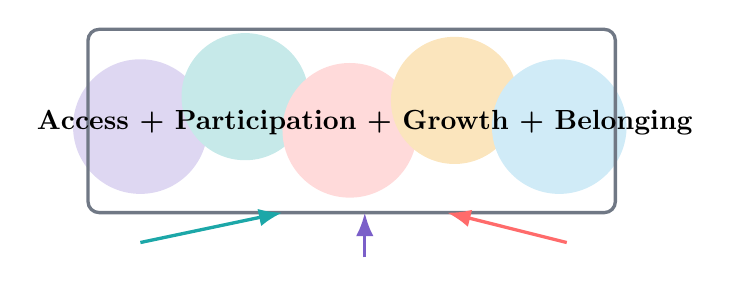
\begin{tikzpicture}[scale=0.95]
  \fill[Purple!25] (-3,0.2) circle (0.9);
  \fill[Teal!25] (-1.6,0.6) circle (0.85);
  \fill[Coral!25] (-0.2,0.15) circle (0.9);
  \fill[Gold!35] (1.2,0.55) circle (0.85);
  \fill[Sky!35] (2.6,0.2) circle (0.9);
  \draw[very thick,Ink!65,rounded corners] (-3.7,-0.95) rectangle (3.35,1.5);
  \node[font=\bfseries,align=center] at (0,0.25) {Access + Participation + Growth + Belonging};
  \draw[-{Latex[length=3mm]},very thick,Teal] (-3,-1.35) -- (-1.1,-0.95);
  \draw[-{Latex[length=3mm]},very thick,Purple] (0,-1.55) -- (0,-0.95);
  \draw[-{Latex[length=3mm]},very thick,Coral] (2.7,-1.35) -- (1.1,-0.95);
\end{tikzpicture}
\end{figure}
\quoteBox{``Inclusion is not working just because students are in the room.''}
\end{frame}

% Slide 2
\begin{frame}
\slideTitle{Today's purpose}
\begin{columns}[T,totalwidth=\linewidth]
\begin{column}{0.52\linewidth}
\begin{itemize}
  \item Reframe evidence beyond placement and task completion.
  \item Notice what gets missed when evidence is too narrow.
  \item Practice designing evidence collection that honors variability.
\end{itemize}
\quoteBox{``The question is not only: Did the student finish? It is: What did the environment allow us to see?''}
\end{column}
\begin{column}{0.43\linewidth}
\begin{figure}
\centering
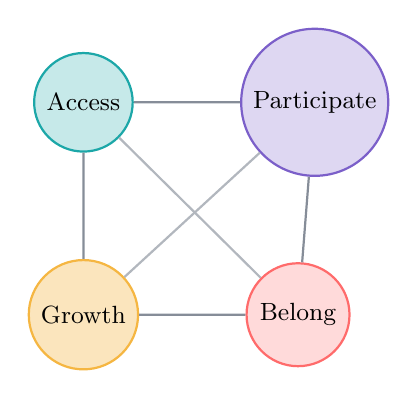
\begin{tikzpicture}[node distance=1.35cm, every node/.style={font=\small}]
  \node[circle,fill=Teal!25,draw=Teal,thick,minimum size=1.15cm] (a) {Access};
  \node[circle,fill=Purple!25,draw=Purple,thick,minimum size=1.15cm,right=of a] (p) {Participate};
  \node[circle,fill=Gold!35,draw=Gold,thick,minimum size=1.15cm,below=of a] (g) {Growth};
  \node[circle,fill=Coral!25,draw=Coral,thick,minimum size=1.15cm,right=of g] (b) {Belong};
  \draw[thick,Ink!55] (a)--(p)--(b)--(g)--(a);
  \draw[thick,Ink!35] (a)--(b);
  \draw[thick,Ink!35] (p)--(g);
\end{tikzpicture}
\end{figure}
\end{column}
\end{columns}
\end{frame}

% Slide 3
\begin{frame}
\slideTitle{Big idea from the reading}
\begin{columns}[T,totalwidth=\linewidth]
\begin{column}{0.52\linewidth}
\large Evidence for inclusion should show more than physical placement.\par
\vspace{0.25cm}
\normalsize It should help us ask whether students are accessing instruction, participating meaningfully, showing growth, and remaining connected to the learning community.
\quoteBox{``A student can be present and still be excluded by what we choose to measure.''}
\end{column}
\begin{column}{0.43\linewidth}
\begin{figure}
\centering
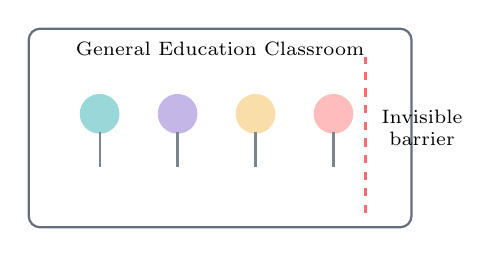
\begin{tikzpicture}[scale=0.9]
  \draw[rounded corners,thick,Ink!70,fill=white] (-2.7,-1.4) rectangle (2.7,1.4);
  \node[font=\scriptsize] at (0,1.12) {General Education Classroom};
  \foreach \x/\c in {-1.7/Teal,-0.6/Purple,0.5/Gold,1.6/Coral}{
    \fill[\c!45] (\x,0.2) circle (0.28);
    \draw[Ink!60,thick] (\x,-0.55) -- (\x,-0.05);
  }
  \draw[very thick,Coral,dashed] (2.05,-1.2) -- (2.05,1.0);
  \node[align=center,font=\scriptsize] at (2.85,0) {Invisible\\barrier};
\end{tikzpicture}
\end{figure}
\end{column}
\end{columns}
\end{frame}

% Slide 4
\begin{frame}
\slideTitle{What can count as evidence?}
\begin{columns}[T,totalwidth=\linewidth]
\begin{column}{0.52\linewidth}
\begin{itemize}
  \item Written products and assessments
  \item Peer explanation and teacher conference notes
  \item Revision, persistence, and strategy shifts
  \item Questions students ask when they get stuck
  \item Belonging, participation, and confidence over time
\end{itemize}
\quoteBox{``The first visible product is not always the strongest evidence of learning.''}
\end{column}
\begin{column}{0.43\linewidth}
\begin{figure}
\centering
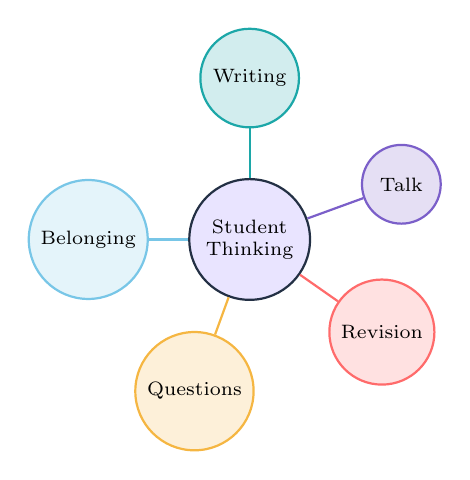
\begin{tikzpicture}[every node/.style={font=\scriptsize,align=center}]
  \node[circle,draw=Ink,fill=Lavender,thick,minimum size=1.25cm] (c) {Student\\Thinking};
  \foreach \name/\ang/\col/\txt in {w/90/Teal/Writing,t/20/Purple/Talk,r/-35/Coral/Revision,q/-110/Gold/Questions,b/180/Sky/Belonging}{
    \node[circle,draw=\col,fill=\col!20,thick,minimum size=1.0cm] (\name) at (\ang:2.05) {\txt};
    \draw[thick,\col] (c)--(\name);
  }
\end{tikzpicture}
\end{figure}
\end{column}
\end{columns}
\end{frame}

% Slide 5
\begin{frame}
\slideTitle{Equity lens: who gets misread?}
\begin{columns}[T,totalwidth=\linewidth]
\begin{column}{0.54\linewidth}
When evidence is narrow, we can confuse access barriers with ability. This is especially risky for students whose processing, language, communication, sensory needs, or cultural expectations do not match the classroom's default rhythm.
\quoteBox{``If we only measure the easiest-to-see behavior, we may miss the hardest-working thinking.''}
\end{column}
\begin{column}{0.41\linewidth}
\begin{figure}
\centering
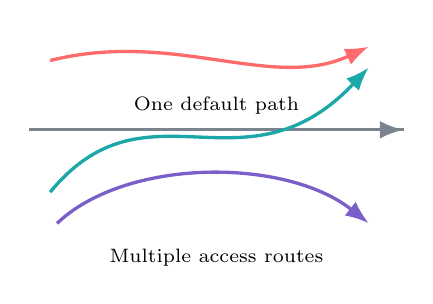
\begin{tikzpicture}[scale=0.88]
  \draw[very thick,Ink!60] (-2.7,0) -- (2.7,0);
  \node[font=\scriptsize] at (0,0.35) {One default path};
  \draw[-{Latex[length=3mm]},very thick,Ink!60] (-2.7,0) -- (2.7,0);
  \draw[-{Latex[length=3mm]},very thick,Teal] (-2.4,-0.9) .. controls (-1,0.8) and (0.4,-1.0) .. (2.2,0.9);
  \draw[-{Latex[length=3mm]},very thick,Purple] (-2.3,-1.35) .. controls (-1.3,-0.4) and (1,-0.4) .. (2.2,-1.35);
  \draw[-{Latex[length=3mm]},very thick,Coral] (-2.4,1.0) .. controls (-0.6,1.45) and (0.8,0.55) .. (2.2,1.2);
  \node[font=\scriptsize,align=center] at (0,-1.85) {Multiple access routes};
\end{tikzpicture}
\end{figure}
\end{column}
\end{columns}
\end{frame}

% Slide 6
\begin{frame}
\slideTitle{Activity 1: Evidence sort}
\begin{columns}[T,totalwidth=\linewidth]
\begin{column}{0.55\linewidth}
\textbf{In pairs or triads:} Sort the examples into three groups.\par
\vspace{0.2cm}
\begin{itemize}
  \item Easy-to-measure evidence
  \item Process evidence
  \item Evidence we often miss
\end{itemize}
\vspace{0.15cm}
Then ask: \textbf{Which students are most likely to be misread if we only use the first group?}
\quoteBox{``Evidence is a design choice before it is a data point.''}
\end{column}
\begin{column}{0.4\linewidth}
\begin{figure}
\centering
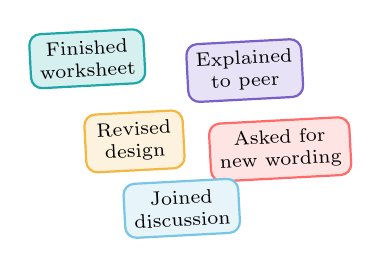
\begin{tikzpicture}[every node/.style={font=\scriptsize,align=center},rotate=0]
  \foreach \x/\y/\c/\txt in {-1.2/0.8/Teal/Finished\\worksheet,0.8/0.65/Purple/Explained\\to peer,-0.6/-0.25/Gold/Revised\\design,1.25/-0.35/Coral/Asked for\\new wording,0/-1.1/Sky/Joined\\discussion}{
    \node[draw=\c,fill=\c!18,thick,rounded corners,minimum width=1.25cm,minimum height=0.62cm,rotate=3] at (\x,\y) {\txt};
  }
\end{tikzpicture}
\end{figure}
\end{column}
\end{columns}
\end{frame}

% Slide 7
\begin{frame}
\slideTitle{Activity 2: Redesign the evidence plan}
\begin{columns}[T,totalwidth=\linewidth]
\begin{column}{0.57\linewidth}
Choose one lesson you teach or remember. Add:
\begin{itemize}
  \item two process checkpoints;
  \item one student voice prompt;
  \item one alternative way to show understanding.
\end{itemize}
\vspace{0.1cm}
\textbf{Prompt:} What would you see now that you might have missed before?
\quoteBox{``A stronger evidence plan does not lower the goal. It gives the goal more ways to become visible.''}
\end{column}
\begin{column}{0.38\linewidth}
\begin{figure}
\centering
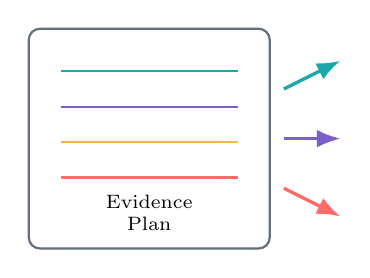
\begin{tikzpicture}[scale=0.9,every node/.style={font=\scriptsize}]
  \draw[rounded corners,thick,Ink!70,fill=white] (-1.7,-1.55) rectangle (1.7,1.55);
  \draw[thick,Teal] (-1.25,0.95) -- (1.25,0.95);
  \draw[thick,Purple] (-1.25,0.45) -- (1.25,0.45);
  \draw[thick,Gold] (-1.25,-0.05) -- (1.25,-0.05);
  \draw[thick,Coral] (-1.25,-0.55) -- (1.25,-0.55);
  \node[align=center] at (0,-1.05) {Evidence\\Plan};
  \draw[-{Latex[length=3mm]},very thick,Teal] (1.9,0.7) -- (2.7,1.1);
  \draw[-{Latex[length=3mm]},very thick,Purple] (1.9,0) -- (2.7,0);
  \draw[-{Latex[length=3mm]},very thick,Coral] (1.9,-0.7) -- (2.7,-1.1);
\end{tikzpicture}
\end{figure}
\end{column}
\end{columns}
\end{frame}

% Slide 8
\begin{frame}
\slideTitle{Leave with this}
\begin{columns}[T,totalwidth=\linewidth]
\begin{column}{0.53\linewidth}
\Large Before concluding that a student did not learn, ask:\par
\vspace{0.2cm}
\normalsize
\begin{itemize}
  \item Did the student have access to the task?
  \item Did we collect evidence across the process?
  \item Did our evidence plan value belonging and participation?
\end{itemize}
\quoteBox{``Look again before you conclude.''}
\end{column}
\begin{column}{0.42\linewidth}
\begin{figure}
\centering
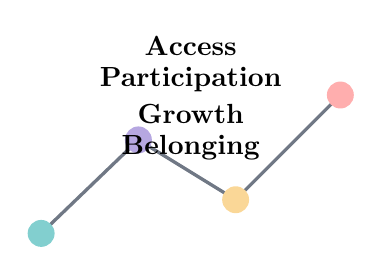
\begin{tikzpicture}[scale=0.95]
  \draw[very thick,Ink!65] (-2,-1) -- (-0.7,0.25) -- (0.6,-0.55) -- (2,0.85);
  \foreach \x/\y/\c in {-2/-1/Teal,-0.7/0.25/Purple,0.6/-0.55/Gold,2/0.85/Coral}{
    \fill[\c!55] (\x,\y) circle (0.18);
  }
  \node[font=\bfseries,align=center] at (0,1.5) {Access};
  \node[font=\bfseries,align=center] at (0,1.05) {Participation};
  \node[font=\bfseries,align=center] at (0,0.6) {Growth};
  \node[font=\bfseries,align=center] at (0,0.15) {Belonging};
\end{tikzpicture}
\end{figure}
\end{column}
\end{columns}
\vspace{0.15cm}
\centering\small Based on ED452C Session 7: Evidence in Support of Inclusive Education.
\end{frame}

\end{document}
